\chapter{Thực nghiệm so sánh trên tập dữ liệu CIFAR}\label{chap:thucnghiemcifar}

Sau khi thử nghiệm việc sử dụng các hàm kích hoạt khác nhau trên tập dữ liệu MNIST, ta vẫn chưa có được một sự chênh lệch lớn nào để có thể dựa vào đó, lựa chọn một hàm kích hoạt phù hợp với các kiến trúc tích chập.
Điều đó khiến ta cần phải thực nghiệm trên một tập dữ liệu khó hơn và với những kiến trúc tích chập khoa học hơn.
Vì thế, tập dữ liệu CIFAR\footnote{The CIFAR-10 and CIFAR-100 dataset, đường dẫn: \href{https://www.cs.toronto.edu/~kriz/cifar.html}{https://www.cs.toronto.edu/~kriz/cifar.html}} được đưa ra huấn luyện và hai tập dữ liệu CIFAR-10 và CIFAR-100 đều sẽ được sử dụng.
Cả 2 tập dữ liệu đều có 50,000 dữ liệu huấn luyện và 10,000 dữ liệu kiểm tra.
Với 50,000 dữ liệu huấn luyện, ta sẽ tách ra ngẫu nhiên 10,000 cho phần dữ liệu kiểm định (tỷ lệ huấn luyện/kiểm định là 8-2).
Tất cả các dữ liệu được làm giàu bằng cách lật đối xứng trục Oy và xoay ảnh một góc nằm trong khoảng $[-2, 2]$ độ.
\vspace{5pt}

Trong phần thử nghiệm này, những kiến trúc được sử dụng là những kiến trúc tích chập hiện đại bao gồm: AlexNet \cite{imagenethinton, alexnetkeras}, SimpleNet \cite{hasanpour2018lets, simplenetkeras} và cuối cùng là VGG16 \cite{simonyan2015deep, vgg16keras}.
Tất cả các tầng tích chập, chuẩn hoá batch, dropout đều sẽ được giữ nguyên theo đúng như kiến trúc gốc.
Chỉ có phần hàm kích hoạt là sẽ thay đổi tất cả thành hàm kích hoạt đang cần thử nghiệm.
Phần kết nối đầy đủ ở cuối sẽ được điều chỉnh sao cho phù hợp với các lớp đầu ra (10 với CIFAR-10 và 100 với CIFAR-100).
Những lớp dày của phần kết nối đầy đủ sẽ sử dụng các loại hàm kích hoạt giống như phần tích chập phía trước của mạng, và sẽ chỉ có mỗi tầng đầu ra là sử dụng hàm kích hoạt softmax để lấy xác suất.

\section{Thực nghiệm các kiến trúc tích chập trên tập dữ liệu CIFAR-10}\label{sec:cifar10}

\begin{table}[ht!]
\centering
\def\arraystretch{1.1}
\begin{tabular}{c|c|c|c|c|c|c|c|c|c|}
\cline{2-10}
                        & \multicolumn{3}{c|}{Mất mát kiểm định} & \multicolumn{3}{c|}{Chính xác kiểm định (\%)} & \multicolumn{3}{c|}{Chính xác kiểm tra (\%)} \\ \cline{2-10} 
                        & Alex     & Simple     & VGG16    & Alex      & Simple     & VGG16     & Alex     & Simple     & VGG16     \\ \hline
\multicolumn{1}{|c|}{$\tanh$} & 1.72        & 0.80          & 3.92     & 62.64        & 73.21         & 10.19     & 62.24       & 72.00         & 10.02     \\ \hline
\multicolumn{1}{|c|}{$\mathcal{R}$} & 1.53        & 0.55          & 2.35     & 64.98        & 80.94         & 79.37     & 65.01       & 80.97         & 79.77     \\ \hline
\multicolumn{1}{|c|}{$\mathcal{R}_L$} & 1.44        & 0.49          & \textbf{2.22}     & 64.66        & 83.30         & \textbf{81.67}     & 64.53       & 83.29         & \textbf{81.92}     \\ \hline
\multicolumn{1}{|c|}{$\mathcal{E}$} & 1.42        & \textbf{0.47}          & 2.62     & 64.62        & \textbf{84.17}         & 74.64     & 65.09       & \textbf{83.48}         & 73.02     \\ \hline
\multicolumn{1}{|c|}{$\mathcal{E}_S$} & 1.37        & 0.59          & 2.43     & 66.47        & 80.91         & 77.21     & 65.99       & 79.52         & 76.49     \\ \hline
\multicolumn{1}{|c|}{$\mathcal{G}$} & 1.33        & 0.58          & 2.31     & \textbf{68.28}        & 80.86         & 79.97     & \textbf{68.27}       & 80.46         & 79.23     \\ \hline
\multicolumn{1}{|c|}{$\mathcal{S}$} & \textbf{1.32}        & 0.83          & 2.33     & 68.01        & 73.94         & 80.11     & 67.69       & 74.18         & 80.31     \\ \hline
\end{tabular}
\caption{Giá trị chính xác (\%) và mất mát của các hàm kích hoạt tương ứng với các kiến trúc mạng tích chập hiện đại trên tập dữ liệu CIFAR-10.}
\label{tab:cifar10}
\end{table}

Biểu đồ giá trị chính xác và mất mát trên tập kiểm định qua mỗi epoch được cho ở các hình \ref{fig:cifar10} và chi tiết về giá trị được cho ở bảng \ref{tab:cifar10}.
\vspace{5pt}

Về giá trị mất mát trên tập kiểm định, kiến trúc AlexNet cho giá trị giảm dần lần lượt từ Tanh (1.72) cho với Swish (1.32).
Dưới ngay Swish là GELU với giá trị mất mát là 1.33.
Còn SimpleNet và VGG16 lại nhận được kết quả thấp nhất của ELU (0.47) và Leaky (2.22).
Những giá trị mất mát phản ánh tốt giá trị xác thực trên tập kiểm định và kiểm tra.
Cụ thể, GELU đạt giá trị chính xác cao nhất mạng Alexnet với 68.28\% trong tập kiểm định và 68.27 trong tập kiểm tra, ngay sát phía sau là Swish với tương ứng 68.01\% và 68.69\%.
ELU và Leaky cho kết quả khá sát nút nhau và nổi trội hơn so với những hàm còn lại.
Với mạng SimpleNet thì ELU đạt giá trị tốt nhất với chính xác 84.17\% kiểm định và 83.48\% kiểm tra.
Về phần Leaky là 81.67\% kiểm định và 81.92\% kiểm tra trong mạng VGG16.
Hàm Tanh lần này không hề cho kết quả tốt khi thực nghiệm trên tập MNIST, thay vào đó cho kết quả tệ nhất ở mọi giá trị trong cả 3 kiến trúc và đặc biệt kiến trúc VGG16 thì hàm Tanh mất khả năng học.
Ngay cả trong một mạng chưa quá sâu như AlexNet, Tanh cũng có dấu hiệu quá khớp khi sau 20 epoch, mất mát trên tập kiểm tra có dấu hiệu đi lên (hình \ref{fig:cifar10b}).
Việc tìm được hố cực tiểu nông của Tanh không còn phát huy so như lúc ở tập dữ liệu MNIST, điều này khiến cho việc dùng hàm Tanh để thử nghiệm không phải là một quyết định sáng suốt.

\begin{table}[ht!]
\centering
\def\arraystretch{1.5}
\begin{tabular}{c|c|c|c|c|c|c|c|}
\cline{2-8}
                        & $\tanh$      & $\mathcal{R}$      & $\mathcal{R}_L$      & $\mathcal{E}$      & $\mathcal{E}_S$      & $\mathcal{G}$      & $\mathcal{S}$      \\ \hline
\multicolumn{1}{|c|}{$\mu_{\text{mất mát}}$} & 2.15  & 1.48  & \textbf{1.38}  & 1.50   & 1.46  & 1.41  & 1.49  \\ \hline
\multicolumn{1}{|c|}{$\mu_{\text{chính xác kiểm định}} (\%)$} & 48.68 & 75.10 & \textbf{76.54} & 74.48 & 74.86 & 76.37 & 74.02 \\ \hline
\multicolumn{1}{|c|}{$\mu_{\text{chính xác kiểm tra}} (\%)$} & 48.09   & 75.25   & \textbf{76.58}   & 73.86   & 74.00   & 75.99   & 74.06   \\ \hline
\end{tabular}
\caption{Giá trị trung bình của các hàm kích hoạt trong 3 kiến trúc tích chập hiện đại trên tập dữ liệu CIFAR-10.}
\end{table}

Không quá bất ngờ khi trung bình của hàm Tanh dưới 50\% khi rõ ràng hàm này không có khả năng học (hình \ref{fig:cifar10e}, \ref{fig:cifar10f}).
Trung bình của Leaky hơn so với các hàm còn lại ở cả 3 đại lượng: mất mát, chính xác kiểm định và chính xác kiểm tra.
Hàm có kết quả tốt thứ nhì là GELU với chênh lệch 0.03 ở giá trị mất mát trung bình $\mu_{\text{mất mát}}$ và giá trị chính xác ở cả 2 tập kiểm tra và kiểm định không quá 0.60\%.
Phần thực nghiệm này RELU không còn mạnh mẽ hơn so với GELU như khi thử nghiệm trên tập MNIST.
Ngoài RELU, hàm ELU cũng không còn được nổi trội, kết quả có được khá cân bằng với Swish khi cả hai đều có giá trị chính xác $\approx 94\%$.

\begin{figure}[ht!]
     \begin{center}
%
        \subfigure[Giá trị chính xác tập kiểm định (A)]{%
            \label{fig:cifar10a}
            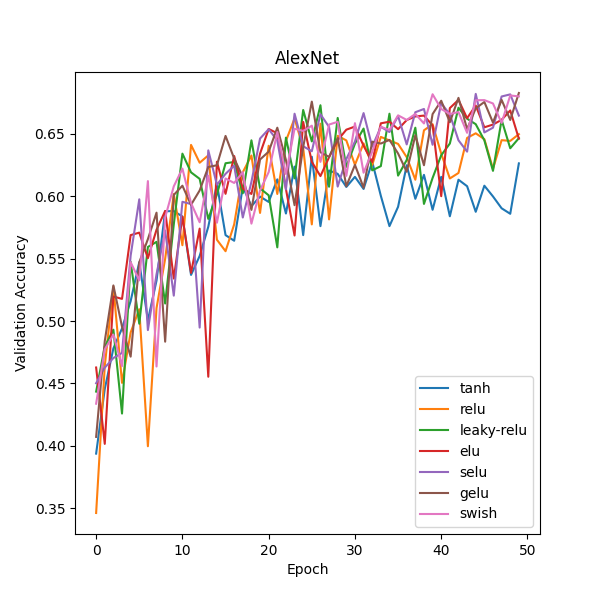
\includegraphics[width=0.4\textwidth]{images/alexnet_acc.png}
        }%
        \subfigure[Giá trị mất mát tập kiểm định (A)]{%
           \label{fig:cifar10b}
           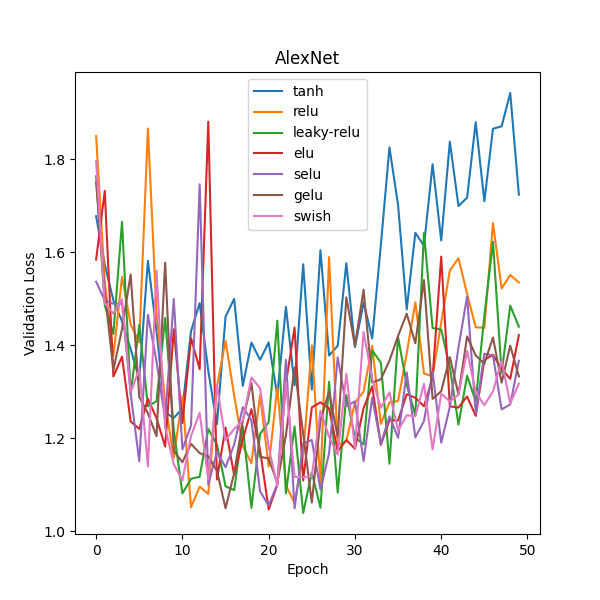
\includegraphics[width=0.4\textwidth]{images/alexnet_loss.png}
        }\\ %  ------- End of the first row ----------------------%
        \subfigure[Giá trị chính xác tập kiểm định (S)]{%
            \label{fig:cifar10c}
            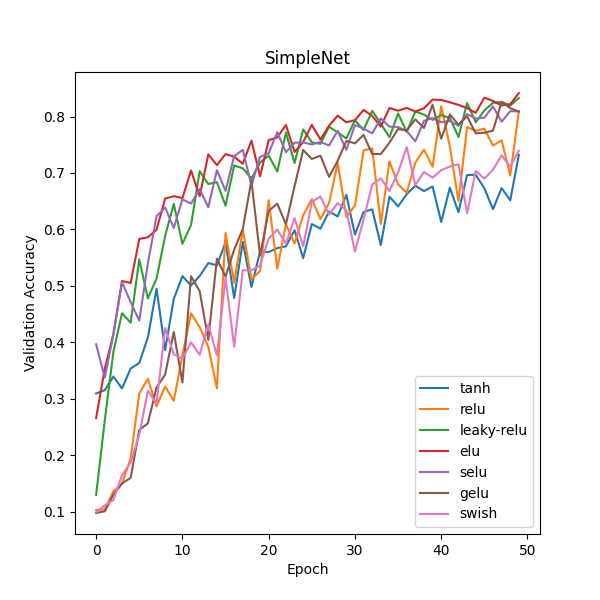
\includegraphics[width=0.4\textwidth]{images/simplenet_acc.png}
        }%
        \subfigure[Giá trị mất mát tập kiểm định (S)]{%
            \label{fig:cifar10d}
            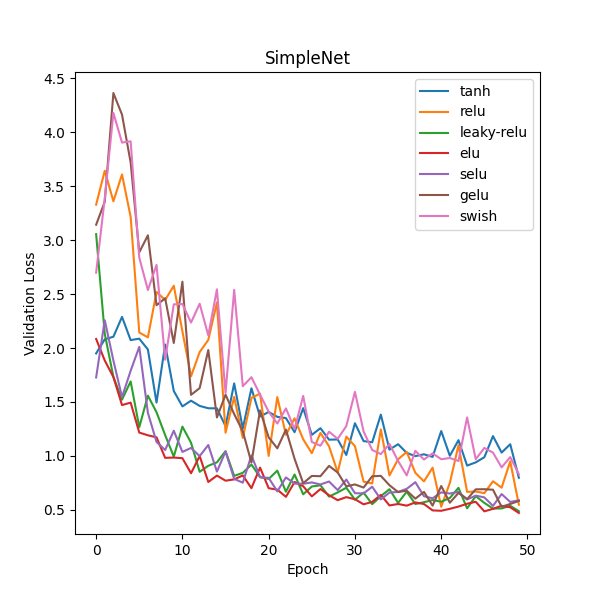
\includegraphics[width=0.4\textwidth]{images/simplenet_loss.png}
        }\\
        %----------------------%
        \subfigure[Giá trị chính xác tập kiểm định (V)]{%
            \label{fig:cifar10e}
            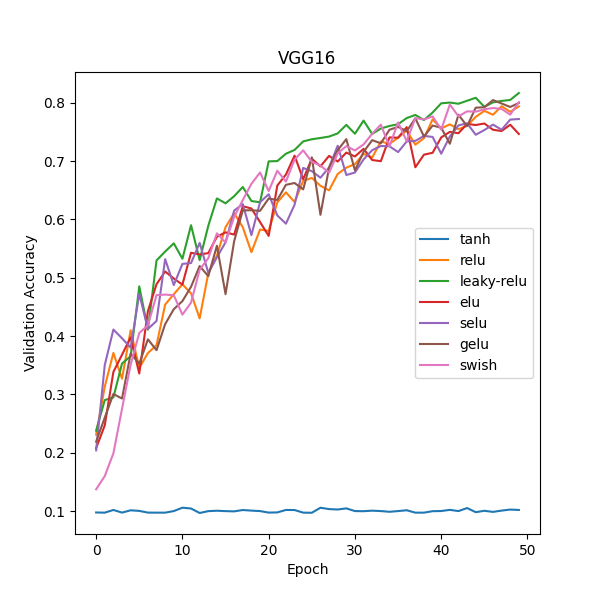
\includegraphics[width=0.4\textwidth]{images/vgg16_acc.png}
        }%
        \subfigure[Giá trị mất mát tập kiểm định (V)]{%
            \label{fig:cifar10f}
            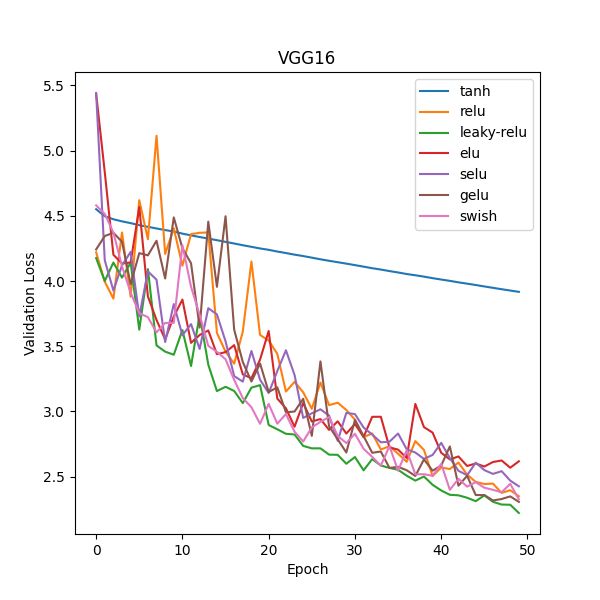
\includegraphics[width=0.4\textwidth]{images/vgg16_loss.png}
        }%
%
    \end{center}
    \caption{%
        Giá trị chính xác và mất mát trên tập kiểm định CIFAR-10 (AlexNet, SimpleNet, VGG16).
     }%
   \label{fig:cifar10}
\end{figure}

\clearpage
\section{Thực nghiệm các kiến trúc tích chập trên tập dữ liệu CIFAR-100}\label{sec:cifar100}

\begin{table}[ht!]
\centering
\def\arraystretch{1.5}
\begin{tabular}{cc|c|c|c|c|c|c|c|}
\cline{3-9}
                                                                                                   &         & $\tanh$     & $\mathcal{R}$     & $\mathcal{R}_L$     & $\mathcal{E}$     & $\mathcal{E}_S$     & $\mathcal{G}$     & $\mathcal{S}$     \\ \hline
\multicolumn{1}{|c|}{\multirow{3}{*}{\begin{tabular}[c]{@{}c@{}}Mất mát\\ kiểm định\end{tabular}}} & AlexNet & 3.83  & 2.96  & 3.07  & 2.76  & \textbf{2.74}  & 3.02  & 3.02  \\ \cline{2-9} 
\multicolumn{1}{|c|}{}                                                                             & SimpleNet       & 4.33  & 2.29  & \textbf{1.76}  & 1.84  & 1.89  & 1.92  & 2.14  \\ \cline{2-9} 
\multicolumn{1}{|c|}{}                                                                             & VGG16       & 6.23  & 4.57  & \textbf{4.27}  & 5.67  & 5.31  & 4.60  & 4.35  \\ \hline
\multicolumn{1}{|c|}{\multirow{3}{*}{\begin{tabular}[c]{@{}c@{}}Top-1\\ kiểm định\end{tabular}}}   & AlexNet & 29.14 & 31.99 & 31.58 & \textbf{38.30} & 38.16 & 35.14 & 34.19 \\ \cline{2-9} 
\multicolumn{1}{|c|}{}                                                                             & SimpleNet       & 12.92 & 40.17 & \textbf{51.92} & 50.91 & 51.86 & 48.58 & 44.54 \\ \cline{2-9} 
\multicolumn{1}{|c|}{}                                                                             & VGG16       & 1.02  & 33.27 & \textbf{37.02} & 26.87 & 27.93 & 34.95 & 34.87 \\ \hline
\multicolumn{1}{|c|}{\multirow{3}{*}{\begin{tabular}[c]{@{}c@{}}Top-3\\ kiểm định\end{tabular}}}   & AlexNet & 47.17 & 50.95 & 49.82 & \textbf{56.96} & 56.60 & 53.51 & 52.22 \\ \cline{2-9} 
\multicolumn{1}{|c|}{}                                                                             & SimpleNet       & 25.40 & 61.53 & \textbf{74.07} & 72.52 & 73.17 & 70.34 & 65.03 \\ \cline{2-9} 
\multicolumn{1}{|c|}{}                                                                             & VGG16       & 2.81  & 54.97 & \textbf{59.79} & 47.61 & 47.76 & 56.87 & 57.35 \\ \hline
\multicolumn{1}{|c|}{\multirow{3}{*}{\begin{tabular}[c]{@{}c@{}}Top-5\\ kiểm định\end{tabular}}}   & AlexNet & 56.08 & 60.04 & 59.32 & \textbf{65.43} & 64.58 & 61.95 & 61.26 \\ \cline{2-9} 
\multicolumn{1}{|c|}{}                                                                             & SimpleNet       & 34.46 & 70.97 & \textbf{81.55} & 80.70 & 81.17 & 78.61 & 73.85 \\ \cline{2-9} 
\multicolumn{1}{|c|}{}                                                                             & VGG16       & 4.62  & 65.67 & \textbf{70.09} & 57.42 & 57.79 & 66.95 & 67.98 \\ \hline
\multicolumn{1}{|c|}{\multirow{3}{*}{\begin{tabular}[c]{@{}c@{}}Top-1\\ kiểm tra\end{tabular}}}    & AlexNet & 29.45 & 32.68 & 30.85 & \textbf{38.39} & 37.46 & 35.42 & 34.87 \\ \cline{2-9} 
\multicolumn{1}{|c|}{}                                                                             & SimpleNet       & 12.80 & 42.25 & \textbf{51.92} & 51.25 & 51.77 & 48.88 & 44.43 \\ \cline{2-9} 
\multicolumn{1}{|c|}{}                                                                             & VGG16       & 1.06  & 33.42 & \textbf{37.51} & 26.25 & 27.68 & 35.47 & 34.96 \\ \hline
\multicolumn{1}{|c|}{\multirow{3}{*}{\begin{tabular}[c]{@{}c@{}}Top-3\\ kiểm tra\end{tabular}}}    & AlexNet & 47.70 & 51.49 & 49.46 & \textbf{57.38} & 56.64 & 53.71 & 52.89 \\ \cline{2-9} 
\multicolumn{1}{|c|}{}                                                                             & SimpleNet       & 25.16 & 64.09 & 72.57 & \textbf{72.81} & 72.11 & 70.09 & 64.55 \\ \cline{2-9} 
\multicolumn{1}{|c|}{}                                                                             & VGG16       & 3.00  & 55.48 & \textbf{60.04} & 45.42 & 46.69 & 57.33 & 57.10 \\ \hline
\multicolumn{1}{|c|}{\multirow{3}{*}{\begin{tabular}[c]{@{}c@{}}Top-5\\ kiểm tra\end{tabular}}}    & AlexNet & 57.04 & 60.68 & 59.27 & \textbf{65.12} & 64.57 & 62.71 & 61.49 \\ \cline{2-9} 
\multicolumn{1}{|c|}{}                                                                             & SimpleNet       & 34.10 & 73.00 & \textbf{80.90} & 50.55 & 80.44 & 78.45 & 73.15 \\ \cline{2-9} 
\multicolumn{1}{|c|}{}                                                                             & VGG16       & 4.99  & 65.45 & \textbf{70.58} & 55.53 & 56.64 & 57.12 & 67.70 \\ \hline
\end{tabular}
\caption{Giá trị mất mát và Top-\{1, 3, 5\} (\%) trên tập kiểm định và kiểm tra CIFAR-100 (AlexNet, SimpleNet, VGG16).}
\label{tab:cifar100}
\end{table}

Số lượng lớp của tập dữ liệu này là 100, khá lớn.
Khi này đánh giá chất lượng ngoài giá trị chính xác, tức Top-1 thì ta cũng nên quan tâm đến Top-3 và Top-5 chính xác.
Biểu đồ giá trị chính xác và mất mát trên tập kiểm định qua mỗi epoch được cho ở các hình \ref{fig:cifar100}, còn Top-3 và Top-5 chín xác trên tập kiểm định sẽ là hình \ref{fig:cifar100top}.
Giá trị chi tiết cho các kết quả trên cho ở bảng \ref{tab:cifar100}.
\vspace{5pt}

Hàm Tanh thêm một lần nữa khẳng định được rằng nó không phù hợp với các mạng tích chập hiện đại khi rất dễ bị quá khớp (hình \ref{fig:cifar100b}), lại không có khả năng học tốt với những mạng tích chập sâu (hình \ref{fig:cifar100c} - \ref{fig:cifar100f}, \ref{fig:cifar100topb} - \ref{fig:cifar100topf}).
Với những hàm khác thì việc học diễn ra khá đúng lộ trình khi càng huấn luyện giá trị chính xác càng lên cao và giá trị mất mát càng giảm.
Dựa vào bảng \ref{tab:cifar100}, ta thấy rằng các chỉ số đánh giá là sự nổi trội của các hàm Leaky và ELU.
Leaky có 13/21 chỉ số đứng đầu, còn ELU là 7/21 chỉ số.
Riêng giá trị mất mát thì SELU mới là hàm đạt giá trị nhỏ nhất.
Chỉ có 3 hàm là Leaky, ELU và SELU mới có giá trị Top-5 kiểm định trên 80\% trong mạng SimpleNet - mạng cho kết quả tốt nhất.
Một điều khá bất ngờ là kết quả Top-5 kiểm tra của ELU lại khá tệ, khi chỉ có 50.55\% (giảm 30.15\%) trong khi 2 hàm vừa nêu vẫn tiếp tục trên 80\% mặc dù đã có giảm sút (dưới 1\%).

\begin{table}[ht!]
\centering
\def\arraystretch{1.5}
\begin{tabular}{c|c|c|c|c|c|c|c|}
\cline{2-8}
                        & $\tanh$      & $\mathcal{R}$      & $\mathcal{R}_L$      & $\mathcal{E}$      & $\mathcal{E}_S$      & $\mathcal{G}$      & $\mathcal{S}$      \\ \hline
\multicolumn{1}{|c|}{$\mu_{\text{mất mát}}$} & 4.80  & 3.27  & \textbf{3.03}  & 3.42   & 3.31  & 3.18  & 3.17  \\ \hline
\multicolumn{1}{|c|}{$\mu_{\text{Top-1 kiểm định}} (\%)$} & 14.36 & 35.14 & \textbf{40.17} & 38.69 & 39.32 & 39.56 & 37.87 \\ \hline
\multicolumn{1}{|c|}{$\mu_{\text{Top-3 kiểm định}} (\%)$} & 25.13   & 55.82   & \textbf{61.23}   & 59.03   & 59.18   & 60.24   & 58.20   \\ \hline
\multicolumn{1}{|c|}{$\mu_{\text{Top-5 kiểm định}} (\%)$} & 31.72   & 65.56   & \textbf{70.32}   & 67.85   & 67.85   & 69.10   & 67.70   \\ \hline
\multicolumn{1}{|c|}{$\mu_{\text{Top-1 kiểm tra}} (\%)$} & 14.44 & 36.12 & \textbf{40.09} & 38.63 & 38.97 & 39.92 & 38.09 \\ \hline
\multicolumn{1}{|c|}{$\mu_{\text{Top-3 kiểm tra}} (\%)$} & 25.29   & 57.02   & \textbf{60.69}   & 58.54   & 58.48   & 60.38   & 58.18   \\ \hline
\multicolumn{1}{|c|}{$\mu_{\text{Top-5 kiểm tra}} (\%)$} & 32.04   & 66.38   & \textbf{70.25}   & 67.07   & 67.22   & 69.43   & 67.45   \\ \hline
\end{tabular}
\caption{Giá trị trung bình của các hàm kích hoạt trong 3 kiến trúc tích chập hiện đại trên tập dữ liệu CIFAR-100.}
\label{fig:meancifar100}
\end{table}

Trong bảng \ref{fig:meancifar100} cho ta thấy rõ ràng khi thực nghiệm trên tập dữ liệu CIFAR-100, Leaky vượt trội hơn khi so sánh với các hàm khác, khi mọi chỉ số đều đứng đầu chứ không chia sẻ bất kỳ vị trí nào.
ELU và SELU cho kết quả khá tương tự nhau và cũng ở mức khá tốt, không thua quá nhiều Leaky như là RELU.
Tuy không cùng họ ELU, nhưng Swish cũng cho kết quả cũng tương đồng với lại ELU và SELU.
Nhưng nếu ta loại bỏ Leaky ra khỏi bảng thì GELU mới là hàm có kết quả vượt trội nhất khi tất cả các giá trị đều đứng đầu.
Nhìn chung, với tập dữ liệu CIFAR-100 thì vẫn là Leaky và GELU cho kết quả ưng ý nhất ở các phương diện đánh giá.

\begin{figure}[ht!]
     \begin{center}
%
        \subfigure[Giá trị chính xác tập kiểm định (A)]{%
            \label{fig:cifar100a}
            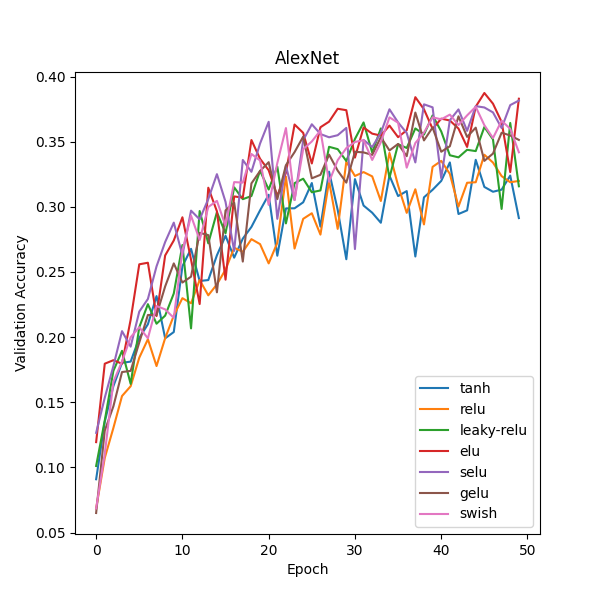
\includegraphics[width=0.4\textwidth]{images/100_alexnet_acc.png}
        }%
        \subfigure[Giá trị mất mát tập kiểm định (A)]{%
           \label{fig:cifar100b}
           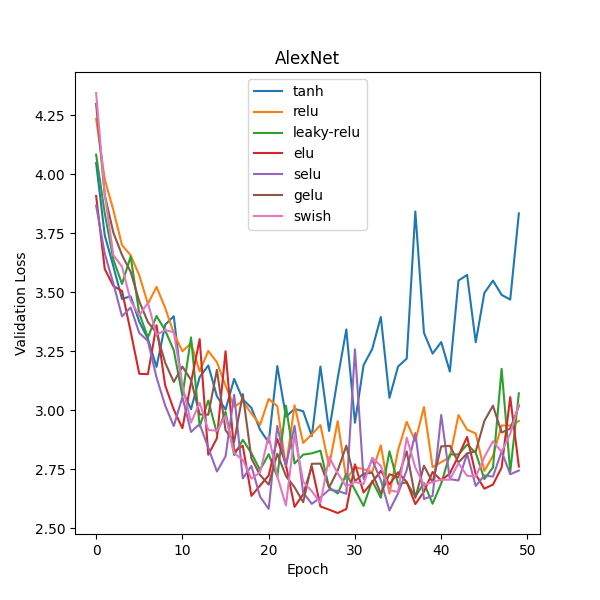
\includegraphics[width=0.4\textwidth]{images/100_alexnet_loss.png}
        }\\ %  ------- End of the first row ----------------------%
        \subfigure[Giá trị chính xác tập kiểm định (S)]{%
            \label{fig:cifar100c}
            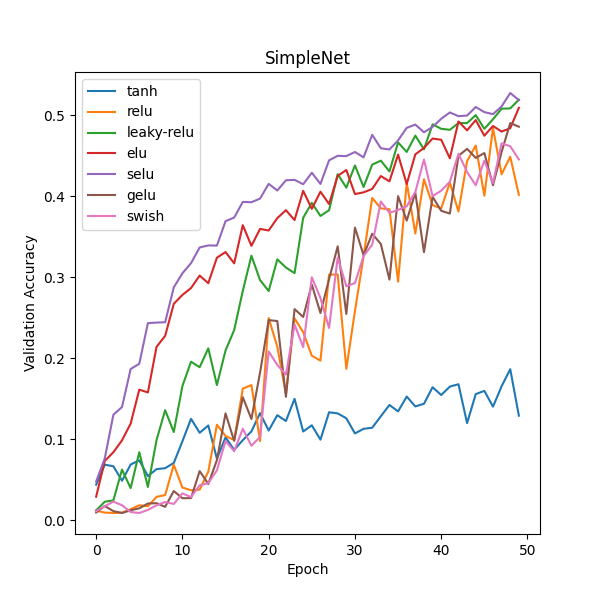
\includegraphics[width=0.4\textwidth]{images/100_simplenet_acc.png}
        }%
        \subfigure[Giá trị mất mát tập kiểm định (S)]{%
            \label{fig:cifar100d}
            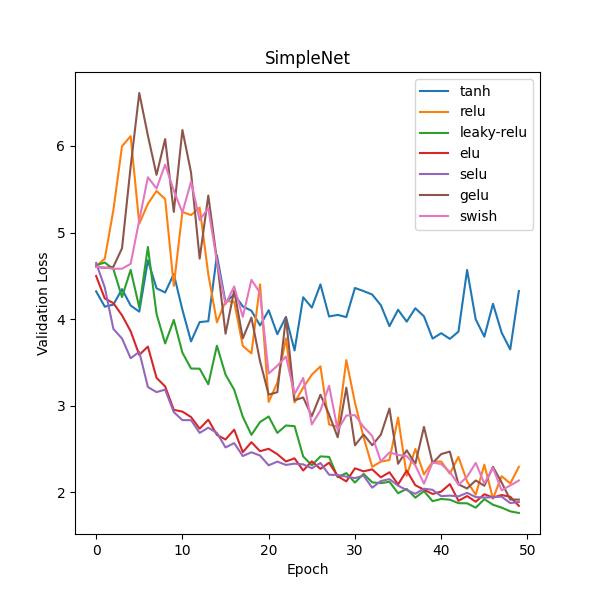
\includegraphics[width=0.4\textwidth]{images/100_simplenet_loss.png}
        }\\
        %----------------------%
        \subfigure[Giá trị chính xác tập kiểm định (V)]{%
            \label{fig:cifar100e}
            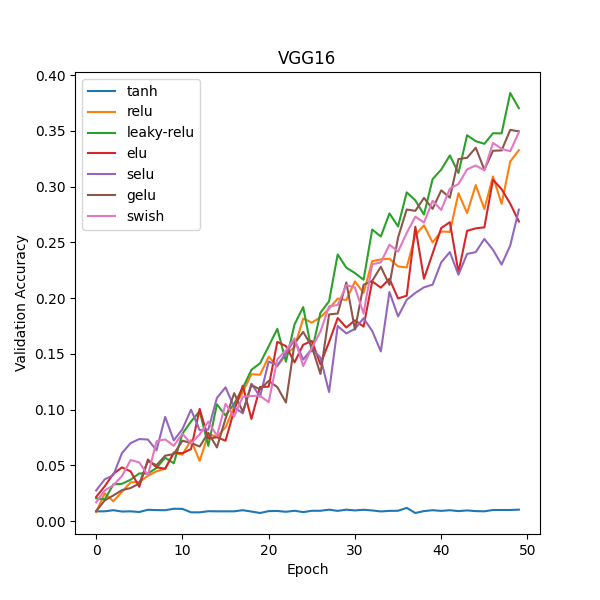
\includegraphics[width=0.4\textwidth]{images/100_vgg16_acc.png}
        }%
        \subfigure[Giá trị mất mát tập kiểm định (V)]{%
            \label{fig:cifar100f}
            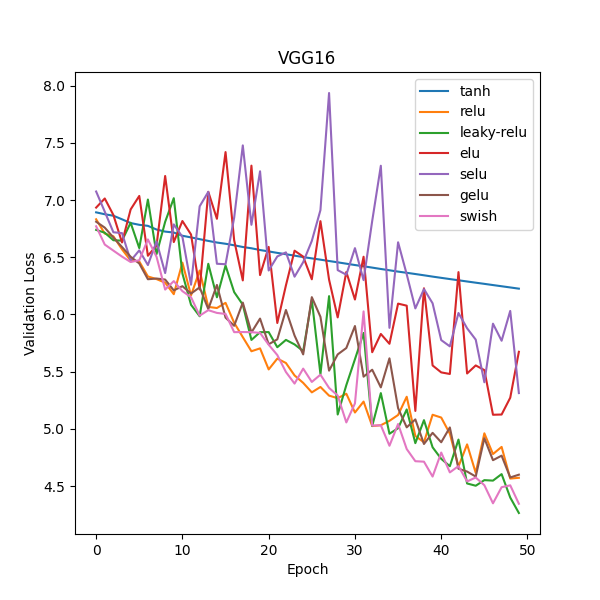
\includegraphics[width=0.4\textwidth]{images/100_vgg16_loss.png}
        }%
%
    \end{center}
    \caption{%
        Giá trị chính xác và mất mát trên tập kiểm định CIFAR-100 (AlexNet, SimpleNet, VGG16).
     }%
   \label{fig:cifar100}
\end{figure}

\begin{figure}[ht!]
     \begin{center}
%
        \subfigure[Giá trị chính xác Top-3 kiểm định (A)]{%
            \label{fig:cifar100topa}
            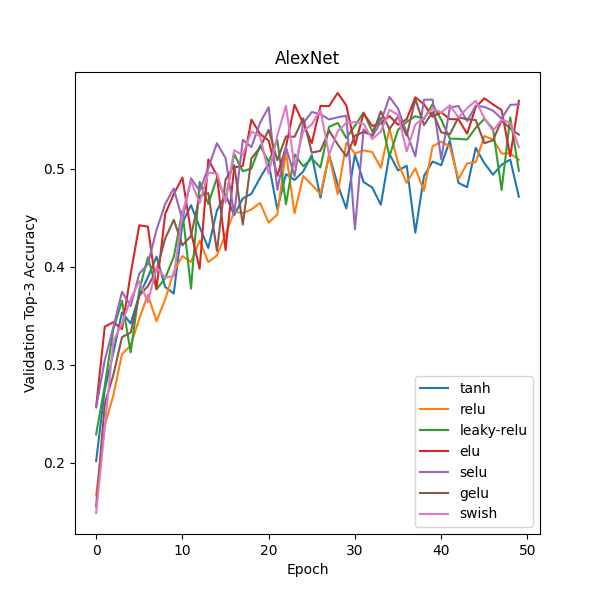
\includegraphics[width=0.4\textwidth]{images/100_alexnet_top3_acc.png}
        }%
        \subfigure[Giá trị chính xác Top-5 kiểm định (A)]{%
           \label{fig:cifar100topb}
           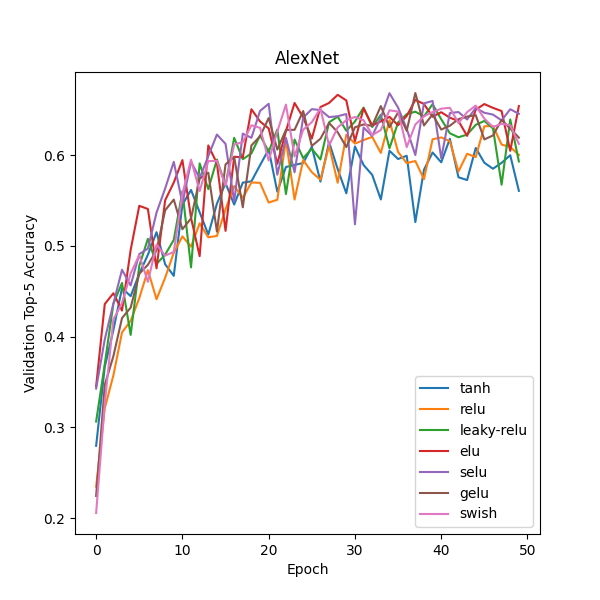
\includegraphics[width=0.4\textwidth]{images/100_alexnet_top5_acc.png}
        }\\ %  ------- End of the first row ----------------------%
        \subfigure[Giá trị chính xác Top-3 kiểm định (S)]{%
            \label{fig:cifar100topc}
            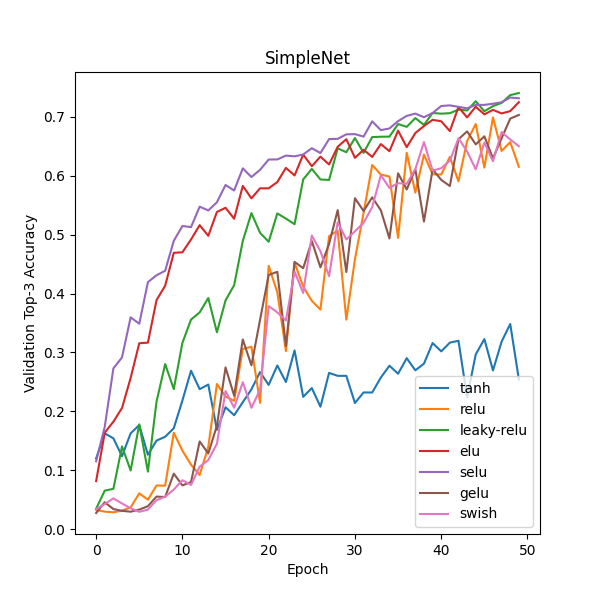
\includegraphics[width=0.4\textwidth]{images/100_simplenet_top3_acc.png}
        }%
        \subfigure[Giá trị chính xác Top-5 kiểm định (S)]{%
            \label{fig:cifar100topd}
            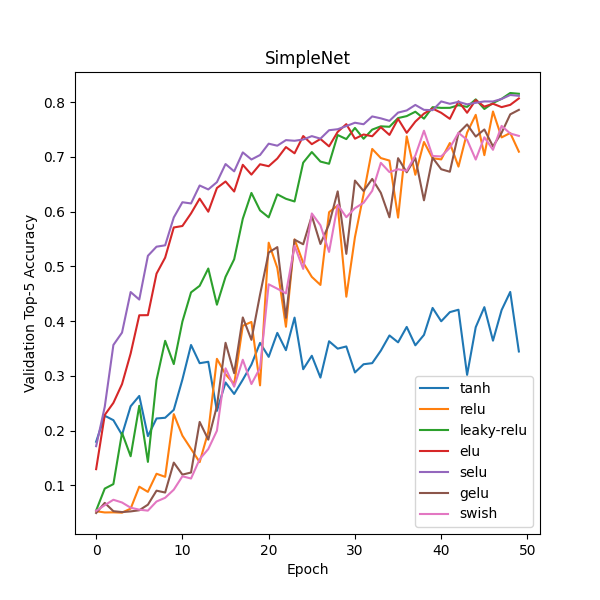
\includegraphics[width=0.4\textwidth]{images/100_simplenet_top5_acc.png}
        }\\
        %----------------------%
        \subfigure[Giá trị chính xác Top-3 kiểm định (V)]{%
            \label{fig:cifar100tope}
            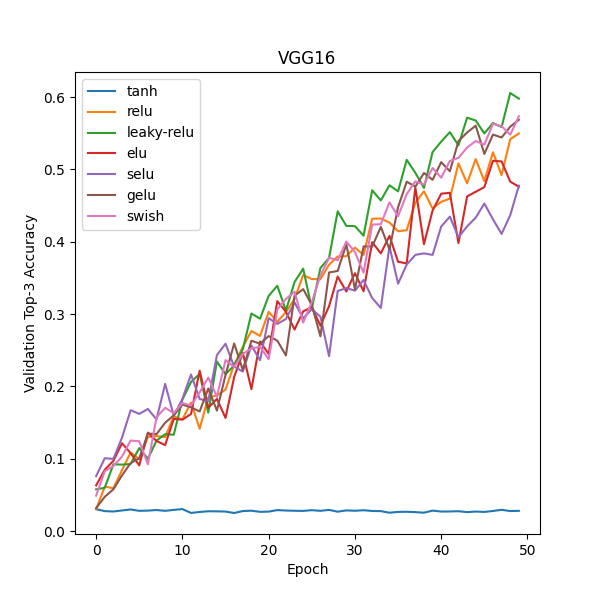
\includegraphics[width=0.4\textwidth]{images/100_vgg16_top3_acc.png}
        }%
        \subfigure[Giá trị chính xác Top-5 kiểm định (V)]{%
            \label{fig:cifar100topf}
            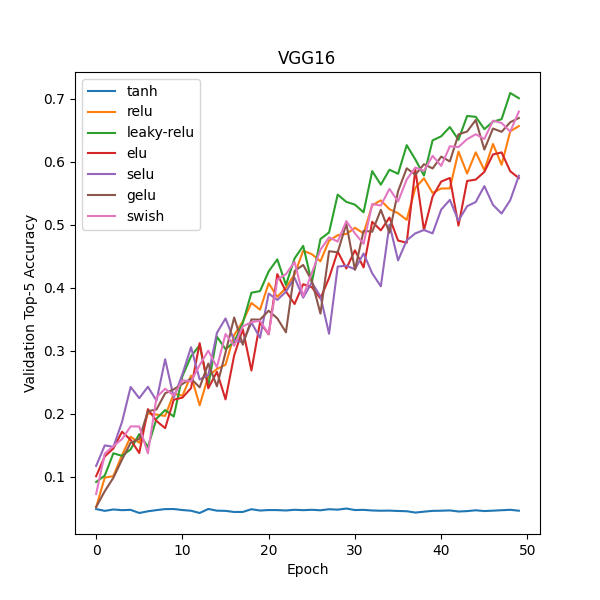
\includegraphics[width=0.4\textwidth]{images/100_vgg16_top5_acc.png}
        }%
%
    \end{center}
    \caption{%
        Giá trị chính xác Top-\{3, 5\} trên tập kiểm định CIFAR-100 (AlexNet, SimpleNet, VGG16).
     }%
   \label{fig:cifar100top}
\end{figure}